% Copyright 2021 Joel Feldman, Andrew Rechnitzer and Elyse Yeager, except where noted.
% This work is licensed under a Creative Commons Attribution-NonCommercial-ShareAlike 4.0 International License.
% https://creativecommons.org/licenses/by-nc-sa/4.0/


 \begin{frame}{Table of Contents }
\mapofcontentsC{\cc}
 \end{frame}
%----------------------------------------------------------------------------------------
%----------------------------------------------------------------------------------------
%----------------------------------------------------------------------------------------
\begin{frame}
For a convergent geometric or telescoping series, we can easily determine what the series converges \textit{to}.\\[1em]

For other types of series, finding out what the series converges to can be very difficult. It is often necessary to resort to approximating the full sum by, for example, using a computer to find the sum of the first $N$ terms, for some large $N$. But before we even try to do that, we should at least know \textit{whether or not the series converges}.
\end{frame}
%----------------------------------------------------------------------------------------
\section{3.3.1 Divergence Test}
%----------------------------------------------------------------------------------------
%----------------------------------------------------------------------------------------
\begin{frame}
\AnswerYes<1>
Suppose a series $\ds\sum_{n=1}^\infty a_n$ converges to a limit $L$.
Let $\ds S_N=\sum_{n=1}^N a_n$.
\begin{alignat*}{2}
\lim_{N \to \infty }S_N&=\sonslide<2->{\color{C3}L}\\
\lim_{N \to \infty }S_{N-1}&=\sonslide<2->{\color{C4}L}\\
\lim_{N \to \infty }\big[ \textcolor{C3}{S_N}-\textcolor{C4}{S_{N-1}}\big]&=\sonslide<2->{L-L=0}\\
\lim_{N \to \infty}a_N&=\sonslide<2->{0}
\end{alignat*}

\begin{center}\begin{tikzpicture}
\foreach \x in {1,...,10}{
	\draw(\x/1.5,0)node[vertex](x\x){};}
\foreach \x in {1,2,3}{
	\draw(x\x)node[below,yshift=-1mm]{$a_\x$};}
\draw(x9)node[below,yshift=-1mm]{$a_{N-1}$};
\draw(x10)node[below,yshift=-1mm]{$a_{N}$};

\draw[decorate,decoration={brace,amplitude=8pt,mirror},C3](0.3,-.5)--(7,-.5)node[midway,below,yshift=-3mm]{$S_N$};

\draw[decorate,decoration={brace,amplitude=8pt},C4](0.3,.5)--(6.3,.5)node[midway,above,yshift=3mm]{$S_{N-1}$};
\end{tikzpicture}\end{center}

\onslide<2-|handout:2>{\alert{Every} convergent series has its $N^{\rm th}$ term, $a_N$, tending to $0$ as $N\rightarrow\infty$.}
\end{frame}
%----------------------------------------------------------------------------------------
%----------------------------------------------------------------------------------------
\begin{frame}
\unote{Theorem~\eref{text}{thm:SRdivergenceTest}}
\begin{block}{Divergence Test}
If the sequence $\left\{ a_n\right\}_{n=c}^\infty$ fails to converge to zero as $n \to \infty$, then the series $\sum\limits_{n=c}^\infty a_n$ diverges.
\end{block}\pause


Do the following series diverge?
\begin{itemize}
\item $\displaystyle\sum\limits_{n=0}^\infty (-1)^n$ \hfill\sonslide<3->{yes, it diverges}
\item $\displaystyle\sum\limits_{n=10}^\infty \left(\frac{1}{10}+\frac{1}{2^n} \right)$
\hfill\sonslide<3->{yes, it diverges}
\item $\displaystyle\sum\limits_{n=15}^\infty \frac{e^n}{2e^n-1}$
\hfill\sonslide<3->{yes, it diverges}
\item $\displaystyle\sum\limits_{n=15}^\infty \frac1n$
\hfill\sonslide<3->{at this point, unclear: maybe, maybe not}
\end{itemize}

\AnswerYes<2>
\end{frame}
%----------------------------------------------------------------------------------------
%----------------------------------------------------------------------------------------


%----------------------------------------------------------------------------------------

%----------------------------------------------------------------------------------------
\begin{frame}
{Using the Divergence Test for ~$\ds\sum a_n$}

\StatusBar{1}{3}
\unote{Warning~\eref{text}{wrn:SRdivTest}}

\centering
\begin{tikzpicture}[node distance = 4cm, auto,inner sep=3mm,->] 
    \node [ellipse,draw] (lim) {$\ds\lim_{n\to \infty}a_n=$ ?}; 
    \onslide<2->{\node [rectangle,draw,below left of=lim] (nonzero) {$\ds\sum a_n$ diverges}; 
    \draw [ultra thick] (lim)--(nonzero)node[midway,left]{$\neq 0$};}
    \onslide<3->{\node [rectangle,draw, below right of=lim] (zero) {\parbox{5cm}{$\ds\sum a_n$ may converge or diverge; use another test}};
    \draw[ultra thick] (lim)--(zero) node[midway,left]{$=0$};
    }
\end{tikzpicture}
\end{frame}
%----------------------------------------------------------------------------------------
%----------------------------------------------------------------------------------------
%----------------------------------------------------------------------------------------
%----------------------------------------------------------------------------------------
\section{3.3.2 Integral Test}
%----------------------------------------------------------------------------------------
\begin{frame}{Harmonic Series: $\sum\limits_{n=1}^\infty\frac1n$}
\sStatusBar{1}{3}
\nsStatusBar{1}{2}
\unote{Example~\eref{text}{eg:firstIntTest}}


\begin{tikzpicture}
\myaxis{x}{0}{9.5}{}{0}{4.5}
\onslide<+->{\ycoord{4}{1}
\ycoord{2}{\frac12}
\ycoord{1.3}{\frac13}
\foreach \x in {1,...,8}{\xcoord{\x}{\x}}
\begin{scope}[xshift=1cm]
\draw[fill=C1] (0,0) rectangle (1,4); %4/1
\draw[fill=C1!50!C2] (1,0) rectangle (2,2); %4/2
\draw[fill=C2] (2,0) rectangle (3,1.3); %4/3
\draw[fill=C2!50!C3] (3,0) rectangle (4,1); %4/4
\draw[fill=C3] (4,0) rectangle (5,.8); %4/5
\draw[fill=C3!50!C4] (5,0) rectangle (6,.67); %4/6
\draw[fill=C4] (6,0) rectangle (7,.57); %4/7
\draw[fill=C4!50!C5] (7,0) rectangle (8,.5); %4/8
\end{scope}}
\onslide<+->{
\draw[very thick, M4] plot[domain=.75:9,smooth](\x,{4/\x})node[above]{$y=\frac{1}{x}$};}
\draw (9,1)node[spoilercolor,above left]{\parbox{4cm}{\begin{align*}
\color{black}\sum_{n=1}^N \frac 1n  & \color{black}\onslide<2->{\geq \int_{1}^{N+1}\frac1x \ \dee x}\\
\sonslide<2->{S_N & \geq \log(N+1)}\\
\sonslide<3->{\lim_{N \to \infty} S_N &= \infty\\
\sum_{n=1}^\infty \frac 1n & \text{ diverges}}
\end{align*}}};
\end{tikzpicture}
\end{frame}
%----------------------------------------------------------------------------------------
\begin{frame}{$\sum_{n=1}^\infty \frac{1}{n}$\qquad diverges}
\begin{tikzpicture}
\weights{1,.5,0.333333,0.25,0.2}
{1,\frac12,\frac13,\frac14,\frac15}
{}
\end{tikzpicture}
\end{frame}
%----------------------------------------------------------------------------------------
%----------------------------------------------------------------------------------------
\begin{frame}{$\sum\limits_{n=1}^\infty\frac1{n^2+1}$}
\sStatusBar{1}{3}
\nsStatusBar{1}{2}
\onslide<+->{}
\begin{tikzpicture}
\myaxis{x}{0}{9.5}{}{0}{4.5}
\foreach \x in {1,...,8}{\xcoord{\x}{\x}}
\ycoord{4}{1}
\ycoord{2}{\frac12}
\ycoord{.8}{\text{\small$\frac15$}}
\ycoord{.4}{\text{\tiny$\frac1{10}$}}
\begin{scope}[xshift=-1cm]
\foreach \a in {1,...,4}{
	\MULTIPLY{\a}{2}{\c}
	\SUBTRACT{\c}{1}{\b}
	\MULTIPLY{\b}{\b}{\bb}
	\ADD{\bb}{1}{\bb}
	\draw[fill=C\a] (\b,0) rectangle (\b+1,4/\bb);
	\ADD{\a}{1}{\ca}
	\MULTIPLY{\c}{\c}{\cc}
	\ADD{\cc}{1}{\cc}
	\draw[fill=C\a!50!C\ca] (\c,0) rectangle (\c+1,4/\cc);}
\end{scope}
%
\draw[very thick, M4] plot[domain=0:1,smooth](\x,{4/(\x*\x+1)});
\draw[very thick, M4] plot[domain=1:9,smooth](\x,{4/(\x*\x+1)})node[above]{$y=\frac{1}{x^2+1}$};
\onslide<2->{\fill[ pattern=north east lines,pattern color=W4] (0,0) --plot[domain=0:9,smooth](\x,{4/(\x*\x+1)});}

\draw (7.5,1.25)node[above left,spoilercolor]{\parbox{4cm}{\[\begin{array}{lcccl}
\onslide<2->{\color{black}0 &\color{black}\leq&}\color{black} \ds\sum_{n=1}^N\frac{1}{n^2+1}&\color{black}\sonslide<2->{\leq&\color{black}\ds \int_0^N \frac{1}{x^2+1}\ \dee x}\\
\sonslide<2->{0 &\leq& S_N & \leq& \arctan(N)}\\[1mm]
\sonslide<3->{0 &\leq& \ds\lim_{N \to \infty}S_N & \leq& \frac{\pi}{2}\\
0 &\leq& \ds\sum_{n=1 }^{\infty}\frac{1}{n^2+1} & \leq& \frac{\pi}{2}\\
 &&\ds\sum_{n=1 }^{\infty}\frac{1}{n^2+1}&&\text{converges}}
\end{array}\]
}};

\end{tikzpicture}
\end{frame}
%----------------------------------------------------------------------------------------
\begin{frame}{$\displaystyle\sum_{n=1}^\infty \frac{1}{n^2+1}$\qquad converges}
\begin{tikzpicture}
\weights{.5,.2,0.1,0.0588235,0.0384615}
{\frac12,\frac15,\frac1{10},\frac1{17},\frac{1}{26}}
{}
\end{tikzpicture}
\end{frame}
%----------------------------------------------------------------------------------------
%----------------------------------------------------------------------------------------
%----------------------------------------------------------------------------------------
\begin{frame}[t]
\unote{Theorem~\eref{text}{thm:SRintegralTest}}
\begin{block}{Integral Test}
Let $N_0$ be any natural number. If $f(x)$ is a function which is defined
and continuous for all $x\ge N_0$ and which obeys
\begin{enumerate}[(i)]
\item $f(x)\ge 0$ for all $x\ge N_0$ and
\item $f(x)$ decreases as $x$ increases and
\item $f(n)=a_n$ for all  $n\ge N_0$.
\end{enumerate}

Then
\hfill\smash{\begin{tikzpicture}[yscale=0.75]
\myaxis{x}{0}{3.25}{y}{0}{1.25}
\xcoord{1}{1}
\xcoord{2}{2}
\xcoord{3}{3}
\draw (1,1)node[vertex,label=above:{$a_1$}]{};
\draw (2,.5)node[vertex,label=above:{$a_2$}]{};
\draw (3,.33)node[vertex,label=above:{$a_3$}]{};
\draw[C1] plot[domain=.8:3.5](\x,{1/\x})node[right]{$y=f(x)$};
\end{tikzpicture}}\begin{equation*}
\sum_{n=1}^\infty a_n\text{ converges }\iff
\int_{N_0}^\infty f(x)\ \dee{x}\text{ converges}
\end{equation*}\pause
Furthermore, when the series converges, the truncation error satisfies
\begin{equation*}
0 \le \sum_{n=1}^\infty a_n-\sum_{n=1}^N a_n\le
  \int_N^\infty f(x)\ \dee{x}\qquad\text{for all $N\ge N_0$}
\end{equation*}

\end{block}
\end{frame}

%----------------------------------------------------------------------------------------
\begin{frame}[t]
\StatusBar{1}{4}
\only<4>{\MoreSpace}
 Does the series $\ds\sum\limits_{n=10}^\infty \frac{1}{n\log n}$ converge or diverge? 
\pause
\onslide<beamer>{\begin{block}{Divergence Test}
If $\lim\limits_{n\to\infty}a_n\neq0$, then $\sum\limits_{n=a}^\infty a_n$ diverges.
\end{block}
\pause
No use here: we need another test.\pause\vfill

Set $f(x)=\frac{1}{x\log x}$.
\begin{enumerate}[(i)]
\item $f(x)\ge 0$ for all $x\ge 10$ and
\item $f(x)$ decreases as $x$ increases and
\item $f(n)=a_n$ for all  $n\ge 10$.
\end{enumerate}\vfill
So, the integral test applies.
}
\end{frame}
%----------------------------------------------------------------------------------------
\begin{frame}<beamer>[t]
\AnswerYes<1>
Does the series $\ds\sum\limits_{n=10}^\infty \frac{1}{n\log n}$ converge or diverge? 

\begin{align*}
\int_{10}^\infty \frac{1}{x\log x}\ \dee x&=
\nsonly{\hspace{6cm}}
\sonslide<2->{
\lim_{b\to\infty}\int_{10}^b \frac{1}{x\log x}\ \dee x
\intertext{Using the substitution $u=\log x$, $\dee u=\frac1x \dee x$,
}
&=\lim_{b\to\infty} \int_{\log(10)}^{\log(b)}\frac{1}{u}\ \dee u\\
&=\lim_{b\to\infty} \big[\log(\log(b))-\log(\log10))\big]=\infty
}
\end{align*}
\sonslide<2->{Since the integral \alert{diverges}, and since $f(x)=\frac{1}{x\log x}$  fulfils the requirements of the integral test, our series \alert{diverges} as well.}
\end{frame}
%----------------------------------------------------------------------------------------
\begin{frame}[t]
Does the series $\ds\sum\limits_{n=10}^\infty \frac{1}{n\log n}$ converge or diverge? 

\begin{tikzpicture}
\myaxis{x}{.2}{9.5}{}{.2}{4.5}
\ycoord{4}{\frac{1}{10\log (10)}}
\ycoord{2}{\frac1{11\log (11)}}
\ycoord{1.3}{\frac1{12\log(12)}}

\foreach \x in {1,...,8}{
\SUBTRACT{\x}{1}{\l}\xcoord{\x}{1\l}}

\begin{scope}[xshift=1cm]
\draw[fill=C1] (0,0) rectangle (1,4); %4/1
\draw[fill=C1!50!C2] (1,0) rectangle (2,2); %4/2
\draw[fill=C2] (2,0) rectangle (3,1.3); %4/3
\draw[fill=C2!50!C3] (3,0) rectangle (4,1); %4/4
\draw[fill=C3] (4,0) rectangle (5,.8); %4/5
\draw[fill=C3!50!C4] (5,0) rectangle (6,.67); %4/6
\draw[fill=C4] (6,0) rectangle (7,.57); %4/7
\draw[fill=C4!50!C5] (7,0) rectangle (8,.5); %4/8
\end{scope}

\draw[very thick, M4] plot[domain=.8:9,smooth](\x,{4/\x})node[above]{$y=\frac{1}{x\log x}$};
\fill[pattern color=W4,pattern=north east lines] (1,0)--plot[domain=1:9,smooth](\x,{4/\x})|-cycle;
\draw[M4] (5,-1.5)node{$\ds\int_{10}^\infty\frac{1}{x\log x}\ \dee x=\infty$};
\end{tikzpicture}
\end{frame}


%----------------------------------------------------------------------------------------
\begin{frame}[t]
\begin{block}{Integral Test, abridged}
... When the series converges, the truncation error satisfies
\[0 \le \sum_{n=1}^\infty a_n-\sum_{n=1}^N a_n  \leq \int _N^\infty f(x) \ \dee x \]
\end{block}\vfill

\begin{tikzpicture}[align=center,yscale=0.5]
\myaxis{x}{0}{8.5}{y}{0}{3.5}
\foreach \x in {1,2,3,4}{
	\MULTIPLY{\x}{2}{\c}
	\SUBTRACT{\c}{1}{\b}
		
	\SQRT{\b}{\d}
	\DIVIDE{1}{\d}{\y}
	\draw[yscale=3,fill=C\x](\b,0) rectangle (\b-1,\y);
	
	\SQRT{\c}{\d}
	\DIVIDE{1}{\d}{\y}
	\ADD{\x}{1}{\xx}
	\draw[yscale=3,fill=C\x!50!C\xx](\c,0) rectangle (\c-1,\y);
	}
\xcoord{3}{N}
\draw[M4,ultra thick]plot[smooth,domain=3: 9]({\x},{3/sqrt(\x)})node[above]{$y=f(x)$};
\fill[pattern=north east lines, pattern color=W4](3,0)--plot[smooth,domain=3: 8.5]({\x},{3/sqrt(\x)})|-cycle;

\draw[ultra thick,decorate,decoration={brace,mirror,amplitude=8pt}] (0,-1.1)--(2.95,-1.1)node[midway,below,yshift=-4mm]{$\ds\sum_{n=1}^Na_n$};
\draw[ultra thick,decorate,decoration={brace,mirror,amplitude=8pt}] (3.05,-1.1)--(9,-1.1)node[midway,below,yshift=-4mm]{$\ds\sum_{n={N+1}}^\infty a_n$ \quad (truncation error)};
\end{tikzpicture}
\end{frame}
%----------------------------------------------------------------------------------------

%----------------------------------------------------------------------------------------
\begin{frame}[t]
\MoreSpace<1>
\AnswerYes<2>
\AnswerSpace

\only<1>{\begin{block}{Integral Test, abridged}
When the series converges, the truncation error satisfies
\[0 \le \sum_{n=1}^\infty a_n-\sum_{n=1}^N a_n \leq \int _N^\infty f(x) \ \dee x \]
\end{block}}


We already decided that the series
$\ds\sum_{n={1}}^{\infty} \frac{1}{n^2+1}$
converges.

Suppose we had a computer add up the terms $n=1$ through $n=100$. Use the integral test to bound the error, $\ds\sum_{n={1}}^\infty \frac{1}{n^2+1}-\sum_{n={1}}^{100} \frac{1}{n^2+1}$.\vfill


\sonslide<3->{
\begin{align*}
&~\sum_{n={1}}^\infty \frac{1}{n^2+1}-\sum_{n={1}}^{100} \frac{1}{n^2+1}\leq 
\int_{100}^\infty \frac{1}{x^2+1}~\dee x\\
&=\lim_{b \to \infty}\left[\arctan(b)-\arctan (100)\right]=
\frac{\pi}{2}-\arctan(100)\approx 0.01
\end{align*}}
\color{black}


\end{frame}
%----------------------------------------------------------------------------------------
\begin{frame}[t]
\AnswerYes<1>\NoSpace<1>
By computer, $\ds\sum_{n=1}^{100}\frac{1}{n^2+1}\approx 1.0667$. Using the truncation error of about 0.01, give a (small) range of possible values for $\ds\sum_{n=1}^{\infty}\frac1{n^2+1}$.


\[
\begin{array}{ccccc}
0 & \leq & \ds\sum_{n={1}}^\infty \frac{1}{n^2+1}-\salert<2->{\sum_{n={1}}^{100} \frac{1}{n^2+1}} & \leq &
\salert<2->{\ds\int_{100}^\infty \frac{1}{x^2+1}~\dee x}
\\
\sonslide<2->{0 &\color{spoilercolor} \leq &\color{spoilercolor} \ds\sum_{n={1}}^\infty \frac{1}{n^2+1}-\alert{1.0667} & \color{spoilercolor}\leq &
\color{spoilercolor}\alert{0.01}
\\[1em]
\color{spoilercolor}1.0667&\color{spoilercolor}\le & \color{spoilercolor}\ds\sum_{n=1}^\infty \frac{1}{n^2+1} &\color{spoilercolor} \le&\color{spoilercolor} 1.0767
}
\end{array}
\]



\end{frame}
%----------------------------------------------------------------------------------------
%----------------------------------------------------------------------------------------
%----------------------------------------------------------------------------------------
%----------------------------------------------------------------------------------------
\begin{frame}{$p$-test}
\AnswerSpace
\AnswerYes<2>
Let $p$ be a positive constant. When we talked about improper integrals, we showed:
\[\int_1^\infty \frac{1}{x^p}\,\dee x \quad\begin{cases}
\text{converges if }p>1\\
\text{diverges if }p\leq1\\
\end{cases}\]
\vfill\pause
Set $f(x)=\dfrac{1}{x^p}$.
\begin{enumerate}[(i)]
\item $f(x)\ge 0$ for all $x\ge 1$, and
\item $f(x)$ decreases as $x$ increases
\end{enumerate}\vfill

\vfill
\[\sum_{n=1}^\infty \frac{1}{n^p}\ \dee x \quad\begin{cases}
\sonslide<3->{\text{converges if }p>1\\
\color{spoilercolor}\text{diverges if }p\leq1}
\end{cases}\]
\unote{Example~\eref{text}{eg:SRpTest}}
\end{frame}
%----------------------------------------------------------------------------------------
%----------------------------------------------------------------------------------------
\begin{frame}[t]
\sStatusBar{1}{3}
\AnswerYes<1-2>
Consider the series
\[\sum_{n=1}^\infty \frac{1}{n^3}	\ .\]
By the $p$-test, we know this series \onslide<2-|handout:0>{converges.}\\[1em]


\onslide<2->{
How many terms should we add up to approximate the series to within an error of no more than $0.02$?
}

\sonslide<3->{
\begin{align*}
\sum_{n=1}^\infty \frac{1}{n^3}-\sum_{n=1}^N\frac{1}{n^3}&\leq
\int_{N}^\infty \frac{1}{x^3}\ \dee x=\lim_{b \to \infty}\left[-\frac{1}{2x^2}\right]_N^b=\frac{1}{2N^2}\\
\frac{1}{2N^2}&\leq \frac{2}{100} \implies N \ge 5
\end{align*}
5 terms will suffice. 
}
\end{frame}
%----------------------------------------------------------------------------------------

%----------------------------------------------------------------------------------------
\begin{frame}
\AnswerYes<6>
$\displaystyle\sum_{n=1}^\infty \frac{1}{n^3}$ converges to within 0.02 of 
$\displaystyle\sum_{n=1}^{5} \frac{1}{n^3}$.

\sonslide<7->{
{$\begin{array}{rcccl}
0 & \leq &\ds \sum_{n=1}^\infty \frac{1}{n^3}-\sum_{n=1}^{5}\frac{1}{n^3} & \leq &0.02\\
0 & \leq &\ds \sum_{n=1}^\infty \frac{1}{n^3}-1.1856 & \leq &0.02\\
1.1856 & \leq &\ds \sum_{n=1}^\infty \frac{1}{n^3} & \leq &1.2056\\
\end{array}$}
\vspace{4cm}} \nsonslide{\vspace{6cm}}

\smash{\begin{tikzpicture}
\weights{1,
0.125,
0.037037037,
0.015625,
0.008}
{1,\frac1{2^3},\frac1{3^3},\frac1{4^3},\frac1{5^3}}
{}
\end{tikzpicture}}
\end{frame}
%----------------------------------------------------------------------------------------
%----------------------------------------------------------------------------------------

%----------------------------------------------------------------------------------------
%----------------------------------------------------------------------------------------
%----------------------------------------------------------------------------------------
\section{3.3.3 Comparison Test}
%----------------------------------------------------------------------------------------
\begin{frame}[t]
\label<3>{note3.3.3a}
\StatusBar{1}{6}
\begin{block}{Observation}
In a series with \textbf{positive} terms, the series either \textbf{converges}, or \textbf{diverges to infinity}. 
\end{block}

If terms are ``too big," series will diverge.\vfill\pause

\hippoindex
\begin{tikzpicture}
\begin{scope}[yshift=-1cm]
\HippoStack{2,0.5,0.2222222222,0.125,0.08,0.0555555556,0.0408163265,0.03125,0.024691358,0.02,0.0165289256,0.0138888889,0.0118343195,0.0102040816,0.0088888889,0.0078125}{}\end{scope}
	
\onslide<3-4>{
{	\color{C1}
	\draw[|-|](-2,-1)--(-2,.75) node[midway,left]{$a_1$};
	\draw[|-|](-1.5,1)--(-1.5,1.5) node[midway,left]{$a_2$};
	\draw[|-|](-.5,1.5)--(-.5,1.75) node[midway,left]{$a_3$};
	}}
\onslide<4>{
	\draw[|-|,very thick,C3] (1.25,-1)--(1.25,2.25)node[near end,right]{$\sum a_n$};}
\end{tikzpicture}\qquad
\onslide<6->{
\smash{\begin{tikzpicture} %%smash will let the hippos float over the text, BUT can't handle line breaks
\VarHippoStack{2,1,0.6666666667,0.5,0.4,0.3333333333,0.2857142857,0.25,0.2222222222,0.2,0.1818181818,0.1666666667,0.1538461538,0.1428571429,0.1333333333,0.125,0.1176470588,0.1111111111,0.1052631579,0.1,0.0952380952,0.0909090909,0.0869565217,0.0833333333,0.08,0.0769230769,0.0740740741,0.0714285714,0.0689655172,0.0666666667,0.064516129,0.0625}{}
\end{tikzpicture}}}

\end{frame}

%----------------------------------------------------------------------------------------
\begin{frame}[t]
$\ds\sum\dfrac{1}{n^2}$ converges\hfill \textcolor{W1}{{$\ds\sum\dfrac{1}{n^2+n}$} \onslide<4->{converges, too}}\\\vfill


\onslide<2->{\begin{tikzpicture} %%smash will let the hippos float over the text, BUT can't handle line breaks
\HippoStack{3,0.75,0.33,0.19,0.12,0.08,0.06,0.05,0.04,0.03,0.02,0.02,0.02,0.02,0.01,0.01,0.01,0.01,0.01,0.01,0.01,0.01,0.01,0.01
}{1,\normalsize $\frac14$,\small $\frac19$}
\onslide<3->{
\begin{scope}[xshift=5cm]
\VarHippoStack{1.5,0.5,0.25,0.15,0.1,0.07,0.05,0.04,0.03,0.03,0.02,0.02,0.02,0.01,0.01,0.01,0.01,0.01,0.01,0.01,0.01,0.01,0.01,
0.01}{$\frac12$,\normalsize$\frac16$,\small $\frac1{12}$}
\end{scope}}%end onslide for second stack
\end{tikzpicture}
}%end onslide
\vfill
\onslide<2->{\parbox{.45\textwidth}{\raggedright Terms are ``small enough" for sum to converge}}\hfill
\onslide<4->{\parbox{.45\textwidth}{\color{W1}\raggedright Terms are also ``small enough" for sum to converge}}
\StatusBar{1}{4}
\end{frame}
%----------------------------------------------------------------------------------------
%----------------------------------------------------------------------------------------

\begin{frame}[t]
\StatusBar{1}{5}
\unote{Therorem~\eref{text}{thm:SRcomparisonTest}}
\begin{block}{The Comparison Test}
Let $N_0$ be a natural number and let $K>0$.
\begin{enumerate}[(a)]
\item If $|a_n| \leq K c_n$ for all $n \ge N_0$ and $\sum\limits_{n=0}^\infty c_n$ converges, then $\sum\limits_{n=0}^\infty a_n$ converges.
\item If $a_n \ge Kd_n \ge 0$ for all $n \ge N_0$ and $\sum\limits_{n=0}^\infty d_n$ diverges, then $\sum\limits_{n=0}^\infty a_n$ diverges.
\end{enumerate}
\end{block}
\pause
Consider $\sum\limits_{n=1}^\infty\frac{1}{n-0.1}$.
\pause
\begin{itemize}[<+->]
	\item We know $0<{\frac{1}{n}}<\textcolor{W1}{ \frac{1}{n-0.1}}$
	\item We know{$\sum\limits_{n=1}^\infty \frac{1}{n}$} diverges (harmonic series)
	\item So, by the comparison test, $\textcolor{W1}{\sum\limits_{n=1}^\infty\frac{1}{n-0.1}}$ diverges as well.
\end{itemize}

\end{frame}
%----------------------------------------------------------------------------------------
%----------------------------------------------------------------------------------------
%----------------------------------------------------------------------------------------
\begin{frame}<beamer>[t]
\centering\vspace{8cm}
\smash{\begin{tikzpicture} %%smash will let the hippos float over the text, BUT can't handle line breaks
\onslide<2->{\HippoStack{2,1,0.67,0.5,0.4,0.33,0.29,0.25,0.22,0.2,0.18,0.17,
0.15,0.14,0.13,0.13,0.12,0.11,0.11,0.1,0.1,0.09,0.09,0.08,0.08,
0.08,0.07,0.07,0.07,0.07,0.06,0.06,0.06,0.06,0.06,0.06,0.05,0.05,
0.05,0.05,0.05,0.05,0.05,0.05,0.04,0.04,0.04,0.04,0.04,0.04,0.04,
0.04,0.04,0.04
}{1,$\frac12$,$\frac13$,\normalsize$\frac14$,\small$\frac15$}}
\begin{scope}[xshift=4cm]
\onslide<3->{\VarHippoStack{2.22,1.05,0.69,0.51,0.41,0.34,0.29,0.25,0.22,0.2,
0.18,0.17,0.16,0.14,0.13,0.13,0.12,0.11,0.11,0.1,0.1,0.09,0.09,0.08,
0.08,0.08,0.07,0.07,0.07,0.07,0.06,0.06,0.06,0.06,0.06,0.06,0.05,0.05,
0.05,0.05,0.05,0.05,0.05,0.05,0.04,0.04
}{$\frac{1}{0.9}$,$\frac{1}{1.9}$,\normalsize$\frac{1}{2.9}$,\small$\frac{1}{3.9}$,\small$\frac{1}{4.9}$}}\end{scope}
\draw (-1,7)node[fill=white,fill opacity=0.75]{$\ds\sum\frac{1}{n}$ diverges};
\onslide<1-3>{\draw[W1](5,7)node[fill=white,fill opacity=0.75]{$\ds\sum\dfrac{1}{n-0.1}$};}
\onslide<4->{\draw[W1](5,7)node[fill=white,fill opacity=0.75]{$\ds\sum\dfrac{1}{n-0.1}$ diverges, too};}
\end{tikzpicture}}%end smash
\end{frame}
%----------------------------------------------------------------------------------------
%----------------------------------------------------------------------------------------
\begin{frame}[t]
\AnswerYes<1,3,5>
\unote{Example \eref{text}{eg:SRcomparisonTestB}}
\sStatusBar{1}{6}
\nsStatusBar{1}{3}
Does the series
$\ds\sum_{n=1}^\infty \frac{n+\cos n}{n^3-1/3}$
converge or diverge?\\
\snshonly{1-2}{1}{1}{\textbf{Step 1: Intuition.}\\  When $n$ is very large, we expect: 
\begin{itemize}
\item $n+\cos n \approx\sonslide<2->{n}$\\[1em]
\item $n^3+\frac13\approx \sonslide<2->{n^3}$\\[1em]
\item So, we expect $\dfrac{n+\cos n}{n^3-1/3} \approx\sonslide<2-> {\dfrac{n}{n^3}=\dfrac{1}{n^2}.}$
\end{itemize}
Since $\ds\sum_{n=1}^\infty\frac{1}{n^2}$\only<1>{ ...} \sonslide<2->{converges (by the $p$-test),}\\
we expect $\ds\sum_{n=1}^\infty \frac{n+\cos n}{n^3-1/3}$ to also
\only<1>{....} \sonslide<2->{converge.}}
%
\snshonly{3-4}{2}{2}{\textbf{Step 2: Choose comparison series.}
\begin{block}{The Comparison Test, abridged}
Let $N_0$ be a natural number and let $K>0$.

If $|a_n| \leq K c_n$ for all $n \ge N_0$ and $\sum\limits_{n=0}^\infty c_n$ converges, then $\sum\limits_{n=0}^\infty a_n$ converges.
\end{block}
To show that original series \alert{converges}, we should find a comparison series that also \alert{converges} and whose terms (times some positive constant) are \alert{larger} than the original terms. \textit{There are many possibilities.} For $n\ge 1$,
\begin{itemize}
\item $n+\cos n <\sonslide<4->{n+n=2n}$
\item $n^3-\frac13>$\sonslide<4->{$n^3-\frac{n^3}{2}=\frac{1}{2}n^3$}
\item So $ \dfrac{n+\cos n}{n^3-1/3}<\sonslide<4->{\dfrac{2n}{\frac12 n^3}=4\cdot\frac{1}{n^2}}$
\end{itemize}
}
%
\snshonly{5-}{3}{3}{\textbf{Step 3: Verify.}
\begin{block}{The Comparison Test, abridged}
Let $N_0$ be a natural number and let $K>0$.

If $|a_n| \leq K c_n$ for all $n \ge N_0$ and $\sum\limits_{n=0}^\infty c_n$ converges, then $\sum\limits_{n=0}^\infty a_n$ converges.
\end{block}

\sonslide<6->{Set $c_n=\frac{1}{n^2}$ and $K=4$. Note $\sum\limits_{n=1}^\infty c_n$ converges.

Note also ${\left|\frac{n+\cos n}{n^3-1/3}\right|<\frac{n+n}{n^3-\frac{n^3}{2}}=4\cdot\frac1{n^2}}$ for all $n \ge 1$.

By the comparison test, $\ds\sum_{n=1}^\infty \frac{n+\cos n}{n^3-1/3}$ converges.}
}


\end{frame}
%----------------------------------------------------------------------------------------
%----------------------------------------------------------------------------------------
%----------------------------------------------------------------------------------------
\begin{frame}<beamer>
\begin{adjustwidth}{-1.5em}{0em}
\begin{tikzpicture}
\onslide<-2>{\draw (-1,7)node{$\ds\sum\frac{1}{n^2}$ converges, so};}
\onslide<1>{
\HippoStack{1,0.25,0.1111111111,0.0625,0.04,0.0277777778,0.0204081633,0.015625,
0.012345679,0.01}{1,\small $\frac14$,\tiny $\frac19$}%1/n^2
}
\onslide<2>{
\foreach \y in {0,1.5,3,4.5}{
\begin{scope}[yshift=\y cm]
\HippoStack{1,0.25,0.1111111111,0.0625,0.04,0.0277777778,0.0204081633,0.015625,
0.012345679,0.01}{}
\end{scope}
}}%copies of 1/n^2
\begin{scope}[xshift=5cm]
\VarHippoStack{4,1,0.4444444444,0.25,0.16,0.1111111111,0.0816326531,0.0625,0.049382716,0.04}{$4\cdot 1$,$4\!\cdot\! \frac14$,\scriptsize $4\!\cdot\! \frac19$, \tiny  $4\!\cdot\! \frac1{16}$}\end{scope}%4/n^2
\draw[W1](5,7)node{$\ds\sum4\cdot \frac{1}{n^2}$ converges\only<-2>{, too}};

\onslide<4->{
\draw (0,7)node{So, $\ds\sum\frac{n+\cos n}{n^3-1/3}$ converges too.};
\HippoStack{2.3104534588,0.2065895431,0.0753752814,0.0525605714,0.042382317,0.0322728143,0.0226281194,0.0153508143,0.0111009191,0.0091639831}{$\frac{1+\cos 1}{1-1/3}$,\small $\frac{2+\cos 2}{8-1/3}$}%\frac{n+\cos n}{n^3-1/3} 
}

\end{tikzpicture}\end{adjustwidth}
\end{frame}
%----------------------------------------------------------------------------------------
%----------------------------------------------------------------------------------------
%--------------------------------

%----------------------------------------------------------------------------------------
\begin{frame}
\label{note3.3.3b}
For the comparison test as we have seen it so far, to conclude that a given series \textcolor{C3}{diverges}, we have to find a divergent comparison series whose terms are \textcolor{C3}{smaller} than (a positive multiple of) those of our original series .
\vfill

\begin{tikzpicture}
\draw[fill=C5, fill opacity=0.1] (0,0) rectangle (3,5);
\draw (1.5,5) node[below]{\fbox{\parbox{2.5cm}{{ \small you must be at least this tall to diverge}}}};
\draw[M4, ultra thick, ->] (1,2.75)--(3,2.75);
\draw (4,-.25) node[above]{
\includegraphics[height=3.5cm]{clipart/holdingsign.png}};
\draw[C3] (3.9,1.75) node{$\sum \frac{1}{n}$};

\onslide<2->{
\draw (6,-.25) node[above]{
\includegraphics[height=4cm]{clipart/holdingsign}};
\draw[C1] (5.9,2) node[]{$\sum \frac{1}{n-\sqrt n}$};}


\onslide<2->{\draw (8,-.25) node[above]{
\includegraphics[height=3cm]{clipart/holdingsign}};
\draw[C2] (7.9,1.6) node[]{\normalsize$\sum \frac{1}{n+\sqrt n}$};}
\end{tikzpicture}
\end{frame}
%----------------------------------------------------------------------------------------
%----------------------------------------------------------------------------------------
%----------------------------------------------------------------------------------------
\begin{frame}
For the comparison test as we've seen it so far, to conclude that a given series \textcolor{C3}{converges}, we have to find a convergent comparison series whose terms are \textcolor{C3}{larger} than (a positive multiple of) those of our original series .\vfill


\hippoindex
\index{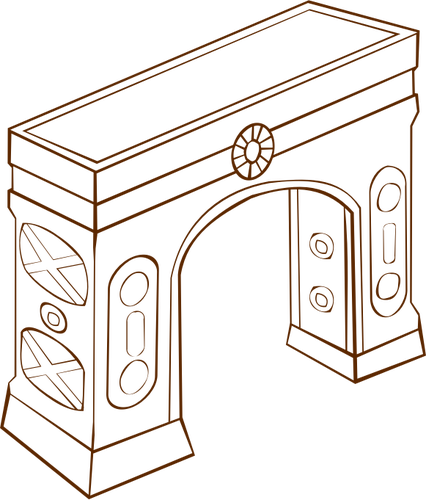
\includegraphics[height=3mm]{clipart/arch}  \href{https://publicdomainvectors.org/en/free-clipart/Vector-illustration-of-role-play-game-map-icon-for-an-arch/22184.html}{Vector illustration of role play game map icon for an arch} is in the Public Domain (accessed Jan 8, 2021)}
\scalebox{0.8}{\begin{tikzpicture}
\draw (0,0)node[above]{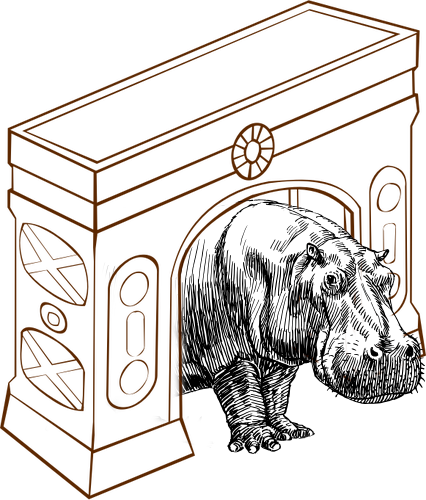
\includegraphics[width=6cm]{clipart/convergent_only}};
\draw(0.45,5.4)node[rotate=23,W2]{\small convergent \qquad series only};
\onslide<2>{\draw (7,0) node[above,xscale=-1]{
\includegraphics[width=4cm]{clipart/hippo2PD}};}
\sonslide<3->{\draw (7,0) node[above,xscale=-1]{
\includegraphics[width=6cm]{clipart/hippo2PD}};}
\sonslide<4->{\draw (0.5,2.75) node[fill=white]{$\ds\sum\frac{1}{n^{3/2}}$};
\draw[W1] (7,3) node[fill=white]{$\ds\sum\frac{1}{n^{3/2}-n}$};}
\end{tikzpicture}}
\end{frame}

%----------------------------------------------------------------------------------------
%----------------------------------------------------------------------------------------
\begin{frame}[t]
\StatusBar{1}{5}
\unote{Theorem \eref{text}{thm:SRlimitComparison}, with a very rough justification}
\begin{block}{Limit Comparison Theorem}
Let $\sum_{n=1}^\infty a_n$ and $\sum_{n=1}^\infty b_n$ be two series with
$b_n>0$ for all $n$. Assume that
\begin{equation*}
\lim_{n\rightarrow\infty}\frac{a_n}{b_n}=L
\end{equation*}
exists.
\begin{enumerate}[(a)]
\item If $\sum_{n=1}^\infty b_n$  converges, then
$\sum_{n=1}^\infty a_n$ converges too.

\item If $L\ne 0$ and $\sum_{n=1}^\infty b_n$  diverges,
then $\sum_{n=1}^\infty a_n$ diverges too.
\end{enumerate}

In particular, \alert<2->{if $L\ne 0$, then $\sum_{n=1}^\infty a_n$ converges
if and only if $\sum_{n=1}^\infty b_n$ converges.}
\end{block}\pause\pause
\begin{itemize}[<+->]
\item For large $n$,~ $a_n \approx L\cdot b_n$;
\item so we expect $\ds\sum a_n$ to behave roughly like $\ds\sum( L \cdot b_n)$;
\item and since $L \neq 0$, we expect $\ds\sum (L \cdot b_n)$ to converge if and only if
$\ds\sum b_n$ converges.
\end{itemize}
\end{frame}
%----------------------------------------------------------------------------------------

%----------------------------------------------------------------------------------------
\begin{frame}[t]
\sStatusBar{1}{3}
\AnswerYes<1-2>
By the $p$-test, $\ds\sum\limits_{n=1}^\infty \frac{1}{n^{3/2}}$ converges. \\
Can we conclude that $\ds\sum\limits_{n=1}^\infty\frac{1}{n^{3/2}-n+1} $ also converges? \sonly{\vfill\vfill}

\sonslide<2->{
\begin{align*}
\color{black}a_n&\color{black}=\frac{1}{n^{3/2}} \qquad b_n=\frac{1}{n^{3/2}-n+1} \\
\sonslide<3->{
\frac{a_n}{b_n}&=\frac{n^{3/2}-n+1}{n^{3/2}}=1-\frac{1}{\sqrt n}+\frac{1}{n^{3/2}}\\
L&=\lim_{n\to\infty}\frac{a_n}{b_n}=1-0+0=1}
\end{align*}\vfill}
\sonslide<3->{Since $L$ is a nonzero real number, the two series either both converge or both diverge. By the $p$-test, $\sum \frac{1}{n^{3/2}}$ converges. So, by the limit comparison test, $\sum\frac{1}{n^{3/2}-n+1} $ also converges.}
\end{frame}
%----------------------------------------------------------------------------------------
%----------------------------------------------------------------------------------------
\begin{frame}<beamer>
\begin{tikzpicture}
\draw (-1,7)node{$\ds\sum\frac{1}{n^{3/2}}$ converges.};
\HippoStack{2.5,
0.8838834765,
0.4811252243,
0.3125,
0.2236067977,
0.1701034544,
0.1349873118,
0.1104854346,
0.0925925926,
0.0790569415,
0.0685253056
}{1,\small $\frac1{\sqrt{2}^3}$,\tiny $\frac1{\sqrt{3}^3}$}%1/n^1.5


\begin{scope}[xshift=5cm]
\VarHippoStack{2.5,
1.3672954017,
0.7821904807,
0.5,
0.3481729332,
0.2578133306,
0.1996763777,
0.1599752538,
0.1315789474,
0.1105080974,
0.094400635
}{1,$\frac{1}{\sqrt{2}^3-1}$,$\frac{1}{\sqrt{3}^3-2}$}\end{scope}%%\frac{n+\cos n}{n^3-1/3} 
\draw[W1] (5,7)node{So, $ \ds\sum\frac{1}{n^{3/2}-n+1}$ converges too.};
\end{tikzpicture}
\end{frame}
%----------------------------------------------------------------------------------------
%----------------------------------------------------------------------------------------
\begin{frame}[t]
\sStatusBar{1}{4}
Does the series $\ds\sum_{n=1}^\infty \frac{\sqrt{n+1}}{n^2-2n+3}$ converge or diverge?
\begin{Ldescription}
\snshonly{-2}{1}{1}{\item[Step 1: Intuition] For large $n$,
\sonslide<2->{ \[\frac{\sqrt{n+1}}{n^2-2n+3}\approx \frac{\sqrt n}{n^2}=\frac{1}{n^{3/2}}\]
So, we'll use $\sum\limits_{n=1}^\infty \frac{1}{n^{3/2}}$ as our comparison series. Since this converges, we expect our original series to converge as well.}}
\snshonly{3-}{2}{2}{\item[ Step 2: Verify Intuition]
Let $a_n=\frac{\sqrt{n+1}}{n^2-2n+3}$ and $b_n=\frac{1}{n^{3/2}}$.
\color{spoilercolor}
\begin{align*}
\color{black}\lim_{n \to \infty}\frac{a_n}{b_n}&=\sonslide<4->{
\lim_{n\to\infty}\frac{\frac{\sqrt{n+1}}{n^2-2n+3}}{\frac{1}{n^{3/2}}}=
\lim_{n\to\infty}\frac{\frac{\sqrt{n+1}}{n^2-2n+3}}{\frac{\sqrt n}{n^{2}}}
\\&=\lim_{n \to \infty}\frac{\sqrt{n+1}\cdot \frac{1}{\sqrt n}}{(n^2-2n+3)\cdot \frac{1}{n^2}}
=\lim_{n \to \infty}\frac{\sqrt{1+\frac{1}{n}}}{1-\frac{2}{n}+\frac{3}{n^2}}\\&=\frac{\sqrt{1+0}}{1+0+0}=1
}
\end{align*}
\sonslide<4->{Since $\sum_{n=1}^\infty \frac{1}{n^{3/2}}$ converges (by the $p$-test), the original series converges as well, by the Limit Comparison Theorem.}}
\end{Ldescription}
\end{frame}
%----------------------------------------------------------------------------------------
%----------------------------------------------------------------------------------------
\begin{frame}<beamer>
\label{note3.3.3c}
\begin{tikzpicture}
\draw (-1,7)node{$\ds\sum\frac{1}{n^{3/2}}$ converges.};
\HippoStack{3,
1.0606601718,
0.5773502692,
0.375,
0.2683281573,
0.2041241452,
0.1619847741,
0.1325825215,
0.1111111111,
0.0948683298
}{1,\small $\frac1{\sqrt{2}^3}$,\tiny $\frac1{\sqrt{3}^3}$}%1/n^3/2


\begin{scope}[xshift=5cm]
\VarHippoStack{2.1213203436,
1.7320508076,
1,
0.6098367211,
0.4082482905,
0.2939723679,
0.2232968783,
0.1764705882,
0.1437398936,
0.1198780045
}{$\frac{1}{\sqrt2}$,$\frac{1}{\sqrt{3}}$,$\frac{1}{3}$,$\frac{\sqrt{5}}{11}$}\end{scope}%%\frac{n+\cos n}{n^3-1/3} 
\draw[W1] (4.5,7)node{So, $\ds\sum \frac{\sqrt{n+1}}{n^2-2n+3}$ converges too.};
\end{tikzpicture}
\end{frame}
%----------------------------------------------------------------------------------------
%----------------------------------------------------------------------------------------
\begin{frame}[t]{Comparison Strategies}
\StatusBar{1}{5}
\begin{itemize}[<+->]
\item Before you can use either comparison test, you need to guess a series to compare. \vfill
\item The series you guess should be easy to deal with.\vfill
\begin{itemize}
\item $p$-series
\item<.-> geometric series
\end{itemize}\vfill
\item Common guess (especially if monotone): consider ``largest" piece of numerator and denominator\\ 
 (constant) $<$ (logarithm) $<$ (polynomial) $<$ (exponential)\vfill
\item After you guess a comparison series, \textbf{show it works} by finding the correct inequality (comparison test), or computing the limit of the ratio (limit comparison test).
\end{itemize}\vfill
\end{frame}
%----------------------------------------------------------------------------------------
%----------------------------------------------------------------------------------------
\begin{frame}[t]{Choose a Series to Compare}
\AnswerYes<1>
\begin{align*}
&\sum_{n=1}^\infty \frac{3n}{n^2+1}  &&
	 \sonslide<2->{\text{One option: } \sum_{n=1}^\infty \frac{3n}{n^2}=\sum_{n=1}^\infty \frac{3}{n}}
	 \\[2em]
& \sum_{n=1}^\infty \frac{n^2+n+1}{n^5-n}  &&
	 \sonslide<2->{\text{One option: } \sum_{n=1}^\infty \frac{n^2}{n^5}= \sum_{n=1}^\infty \frac{1}{n^3}}
	 \\[2em]
&\sum_{k=1}^\infty \frac{k(2+\sin k)}{k^{\sqrt2}} &&
	 \sonslide<2->{\text{One option: } \sum_{k=1}^\infty \frac{2k}{k^{\sqrt 2}}=\sum_{k=1}^\infty \frac{2}{k^{\sqrt 2-1}}}
	 \\[2em]
&\sum_{m=1}^\infty \frac{3m+\sin\sqrt{m}}{m^2}
	&& \sonslide<2->{\text{One option: } \sum_{m=1}^\infty \frac{3m}{m^2}=\sum_{m=1}^\infty \frac{3}{m}}
\end{align*}
\end{frame}
%----------------------------------------------------------------------------------------
%----------------------------------------------------------------------------------------
%----------------------------------------------------------------------------------------
%----------------------------------------------------------------------------------------

%----------------------------------------------------------------------------------------
